\section{Spatial Filtering}

\subsection{Task 1: Theory}
\subsubsection*{a)}
Sampling is the process of converting a continuos-time signal to a discrete-time signal, usually by measuring the continuos-time signal at specific points in time and extending this measurement over a set time step. 

\subsubsection*{b)}
Quantization is the process of constraining a signal from a larger to a smaller set of values, like mapping colours to the standard RGB range of 256 integer values. 

\subsubsection*{c)}
A high contrast image histogram would look similar to a dirac delta function, with most values grouped together around the same intensity.

\subsubsection*{d)}
\begin{table}[]
    \label{tab:initial_image}
    f = \begin{tabular}{|l|l|l|l|l|}
        \hline
        5 & 0 & 2 & 3 & 4 \\ \hline
        3 & 2 & 0 & 5 & 6 \\ \hline
        4 & 6 & 1 & 1 & 4 \\ \hline
    \end{tabular}
\end{table}
\begin{align*}
    n_{\text{pixel}} &= 3 * 5 = 15 \\
    L = 7
    i_0 &= 2 \\ 
    i_1 &= 2 \\
    i_2 &= 2 \\
    i_3 &= 2 \\
    i_4 &= 3 \\
    i_5 &= 2 \\
    i_6 &= 2 \\
    i_7 &= 0
\end{align*}
Then using \cref{eq:equalizer} on \cref{tab:initial_image} gives \cref{tab:equalized_image}. 

\begin{align*}
    \begin{bmatrix}
        n   & 0             & 1             & 2             & 3             & 4             & 5             & 6             & 7 \\ \hline
        f_n &\frac{2}{15} &\frac{2}{15} &\frac{2}{15} &\frac{2}{15} &\frac{3}{15} &\frac{2}{15} &\frac{2}{15} &\frac{0}{15} \\
        F_n &\frac{2}{15} &\frac{4}{15} &\frac{6}{15} &\frac{8}{15} &\frac{11}{15} &\frac{13}{15} &\frac{15}{15} &\frac{15}{15} \\
        E_q & 0 & 1 & 2 & 3 & 4 & 5 & 6 & 6
    \end{bmatrix}
\end{align*}

\begin{equation}
    \label{eq:equalizer}
    g_{i,j} = floor((L - 1) * \sum_{n = 0}^{f_{i,j}} \frac{i_n}{n_{\text{pixel}}}) = floor((L - 1) * F_n)
\end{equation}

\begin{table}[]
    \label{tab:equalized_image}
    \begin{tabular}{|l|l|l|l|l|}
        \hline
        6 & 0 & 2 & 3 & 4 \\ \hline
        3 & 2 & 0 & 5 & 6 \\ \hline
        4 & 6 & 1 & 1 & 4 \\ \hline
    \end{tabular}
\end{table}

\subsubsection*{e)}
The log transform will increase the output intensity for low input intensities, and flatten for high input intensities. This will make it easier to see the lower ranges of the input intensities. If we then apply this transform to 


\newpage
\subsection{Task 2: Programming}
\subsubsection*{a)}
See the result from \cref{fig:greyscale}. 
\begin{figure}[]
    \centering
    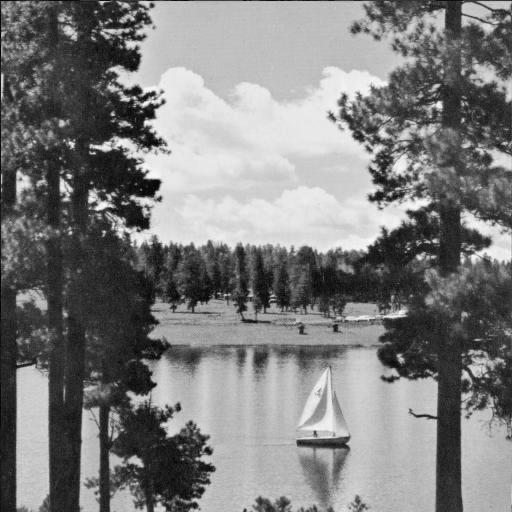
\includegraphics[width=1.00\textwidth]{figures/image_processed/lake_greyscale.jpg}
    \caption{The grey scale version of the lake image}
    \label{fig:greyscale}
\end{figure}

\subsubsection*{b)}
Se the result from \cref{fig:inverse}. 
\begin{figure}[]
    \centering
    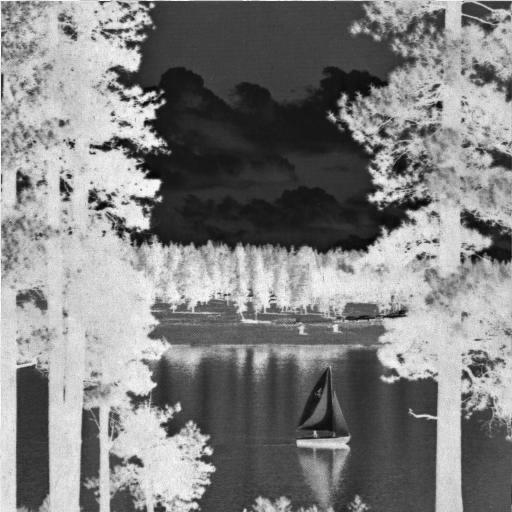
\includegraphics[width=1.00\textwidth]{figures/image_processed/lake_inverse.jpg}
    \caption{The inverse of the grey scale version of the lake image}
    \label{fig:inverse}
\end{figure}

\subsubsection*{c)}
See the results from \cref{fig:convolution_h_a} and \cref{fig:convolution_h_b}.

\begin{figure}[]
    \centering
    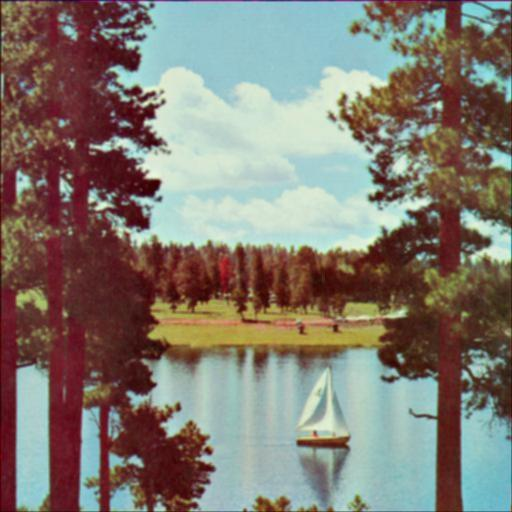
\includegraphics[width=1.00\textwidth]{figures/image_processed/convolved_im_h_a.jpg}
    \caption{Convolution of the lake image with the kernel $h_a$.}
    \label{fig:convolution_h_a}
\end{figure}

\begin{figure}[]
    \centering
    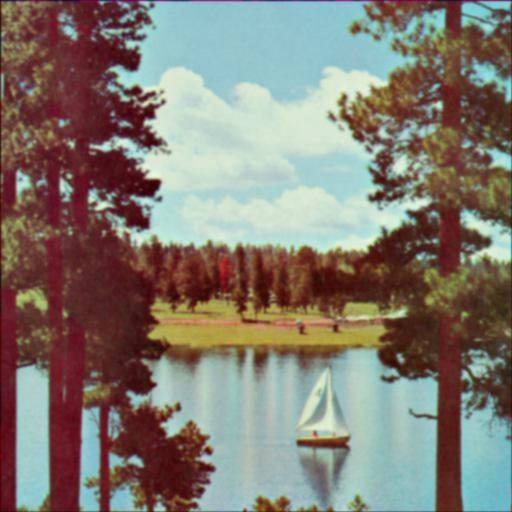
\includegraphics[width=1.00\textwidth]{figures/image_processed/convolved_im_h_b.jpg}
    \caption{Convolution of the lake image with the kernel $h_b$.}
    \label{fig:convolution_h_b}
\end{figure}
